\newpage
\section{RESULTS AND ANALYSIS}


\subsection{Dataset pre-processing}

\subsubsection{Genre Dataset}
In \cite{Downie2003}, Downie presents the problem of a lack of a proper baseline dataset for the AMGC problem, which meant research teams couldn’t scientifically compare and contrast their different approaches.\\
\\
However, the publicly available GTZAN dataset introduced in \cite{Tzanetakis2002}, solved most parts of the issue by soon becoming the standard dataset used by researchers across the world. We too used this dataset for this project. The dataset contains 100 representative excerpts from ten different genre. They were taken from radio, compact disk, and MP3 compressed audio files. All the files are stored as 22 050 Hz, 16-bit, mono audio files. The Genres dataset has the following classes: classical, country, disco, hiphop, jazz, rock, blues, reggae, pop, metal. Among them we were only concerned with five genre as mentioned in Chapter 1: classical, hiphop, jazz, rock, and pop, So, we had a total of 500 songs in our dataset.

\subsubsection{Mood Dataset}
Due to the high variability in the emotional models adopted (whether categorical or dimensional), there have been no popular baseline dataset for MER task.\\
\\
So, to tackle the issue, in 2013, Soleymani et al. \cite{Soleymani2013} created a 1000 songs dataset for emotional analysis of music which uses the Valence-Arousal axes for representing emotional values for songs.\\
\\
The songs, in the dataset, each 45 seconds long, were collected from FMA. They used Amazon Mechanical Turk as a crowdsourcing platform for collecting more than 20,000 annotations on the 1,000 songs.\\
\\
Furthermore, their analysis on the annotations revealed a higher agreement in arousal ratings compared to the valence ratings.\\
\\
We have used a filtered version (with some redundancies removed) of that dataset resulting in a final set of 744 songs. We further labeled them as high/low arousal and high/low valence songs based on the numerical values in the dataset. To achieve equal number of songs in each class, we finally used 600 songs of those 744 songs. 

\subsection{Testing and Validation}
While building a software product, the concept of testing and validation plays an important role throughout its development.
Along with the development of a software product, numerous testing and validation are need to be performed regulary.
In fact, most of the development period is given to testing and validation. It's important as it conforms to whether we are building
product right and whether we are building the right product. After series of testing and validation only we can point that the system
conforms to the desired specifications and need.\\
\\
Since our software project is also research oriented, so we need series of rigorous testing. Not only this, being a predictive system/model
a type of validation and measure for performance is a must, so that it can analyze the result and decide how to progress further accounting the fact.
For our system, we chose cross-validation after we confronted it's popularity for a predictive model and ease of use. Similarly for measure of performance we chose recall, presicion 
and F-measure.\\

\subsubsection{Cross-validation}
Cross-validation is a technique for estimating the performance of a predictive model.
Cross-validation, sometimes called rotation estimation is a model validation technique for assessing how the
results of a statistical analysis will generalize to an independent data set. In a predictive problem like our project, a model is usually given a dataset of known data(training dataset) on which 
the model is trained, and a dataset of unknown data (or first seen data) against which the model is tested (testing dataset). The goal of cross validation is to define a dataset
to "test" the model in the training phase(validation dataset), in order to limit problems like overfitting, give an insight on how the model will generalize to an independent dataset(and unknown dataset, for instance from 
a real problem),etc.\\
\\
One of the main reasons for using cross-validation instead of using the conventional validation is that there is not enough data available to partition it into separate training and test sets without losing
significant modelling or testing capability. There are several cross-validation method out there like leave-p-out cross-validation, leave-one-out cross validation,2-fold cross validaiton, repeated random 
sub-sampling validation, etc. But we decide to got with k-fold cross validation. The main reason for this selection is that k-fold cross-validation estimator can prove to have a lower variance than a single hold-out set 
estimator if the amount of data available is limited. Our main goal with k-fold cross validation is to estimate the expected level of fit of a model to a dataset that is independent of the data that were
used to train the model.\\
\\
In k-fold cross-validation, the original sample is randomly partitioned into k equal sized subsamples. Of the k subsamples,
a single subsample is retained as the validation data for testing the model, and the remaining k - 1 subsamples are used as training
data. The cross-validation process is then repeated k times (the folds), with each of the k subsamples used exactly once as the validation data. The k results from the
folds can then be averaged to produce a single estimation. The advantage of this method over repeated random sub-sampling (see below) is that all
observations are used for both training and validation, and each observation is used for validation exactly once. ten-fold cross-validation is currently
applied in our system. Our music data set is first divided into ten equal samples of songs, and on every run for ten times, a different sample of songs are used for
testing and the rest for training.\\
\\
This k-fold validation validation process is applied with each performance metrics and the appropriate features are taken to classify in our system.

\subsubsection{Measure of Performance}
In a predictive problem, we always need a measure of performance for that predictive model along with cross validation. Based on the value of different attributes falling under 
the measure of performance, we can then have the knowledge of how well the system is performing. It is important because as a matter of fact it provides much deeper insight of the performance of
the predictive model, not only accuracy.\\
\\
Our measure of performance include precision, recall and F-measure. We can say our measure of performance are based on the relevant and non-relevent documents. In this case,
relevant documents are those one which simply belong to the relevant category. Relevant category is also called the true positives. True positive is the number of items correctly
labeled as belong to the positive class or say which are predicted correctly. The not relevant documents are those one which simply are not relevant to the category or say they are false negative. 
False negative is the number of negative items which are predicted to fall under the positive class. False Positive is the number of negative items which are predicted to be in true class.
Similarly, true negative is the number of negative items which are correctly predicted to fall under negative class.

\begin{itemize}
        \item \textbf{Precision}\\
                The precision of a measurement system, related to reproducibility and repeatability, is the degree to which repeated measurements under unchanged
                conditions show the same results. In a classification task, the precision for a class is the number of true positives divided by the total number of elements labeled as 
                belonging to the positive class. A perfect precision score of 1.0 means that every result retrieved by a search was relevant which means falling to the specified class.
                But precision does not say whether all items of that class were correctly predicted.
                \begin{equation}
                        Precision = \frac{True Positive}{True Positive + False Positive}
                \end{equation}
        \item \textbf{Recall}\\
                Recall literally is how many of the true positives were recalled (found), i.e. how many of the correct hits were also found. Recall is also sometimes called sensitivity or probability of detection.
                It is the true positive rate as it measure the proportion of positives that are correctly identified as such. Recall is the number of true positives divided by the total number of elements
                that actually belong to the positive class. A perfect recall score of 1.0 means that all relevant documents were retrieved by search. We can also say that perfect recall shows that all items of a
                class were labeled fall under same class. But recall does not say that how many other items were misclassified to fall under same class.
                \begin{equation}
                        Recall = \frac{True Positive}{True Positive + False Negative}
                \end{equation}
        \item \textbf{F measure}
               A measure that combines precision and recall is the harmonic mean of precision and recall. 
                F measure is the weighted harmonic mean of its the precision and recall of a system. It is sometimes called as balanced F-score. This measure is approximately the average of the two when they are close, and is more generally
                the harmonic mean which for the case of two numbers coincides with the square of the geometric mean divided by the arithmetic mean. There are several reasons that the F-score can be criticized in particular 
                circumstances due to its bias as an evaluation metric. This is also known as the $F_1$ measure, because recall and precision are evenly weighted.
                \begin{equation}
                        F = 2*\frac{Precision*Recall}{Precision+Recall}
                \end{equation}
        \end{itemize}
        All three performance metrics have been used to determine the best features to be used for classification in cases of genre, arousal and valence.

\subsection{Audio Pre-processing}
\subsubsection{Effect of Window Functions}
We tried out five window functions to smoothen the data frames obtained from the samples. 

\begin{figure}[h!]
        \centering
        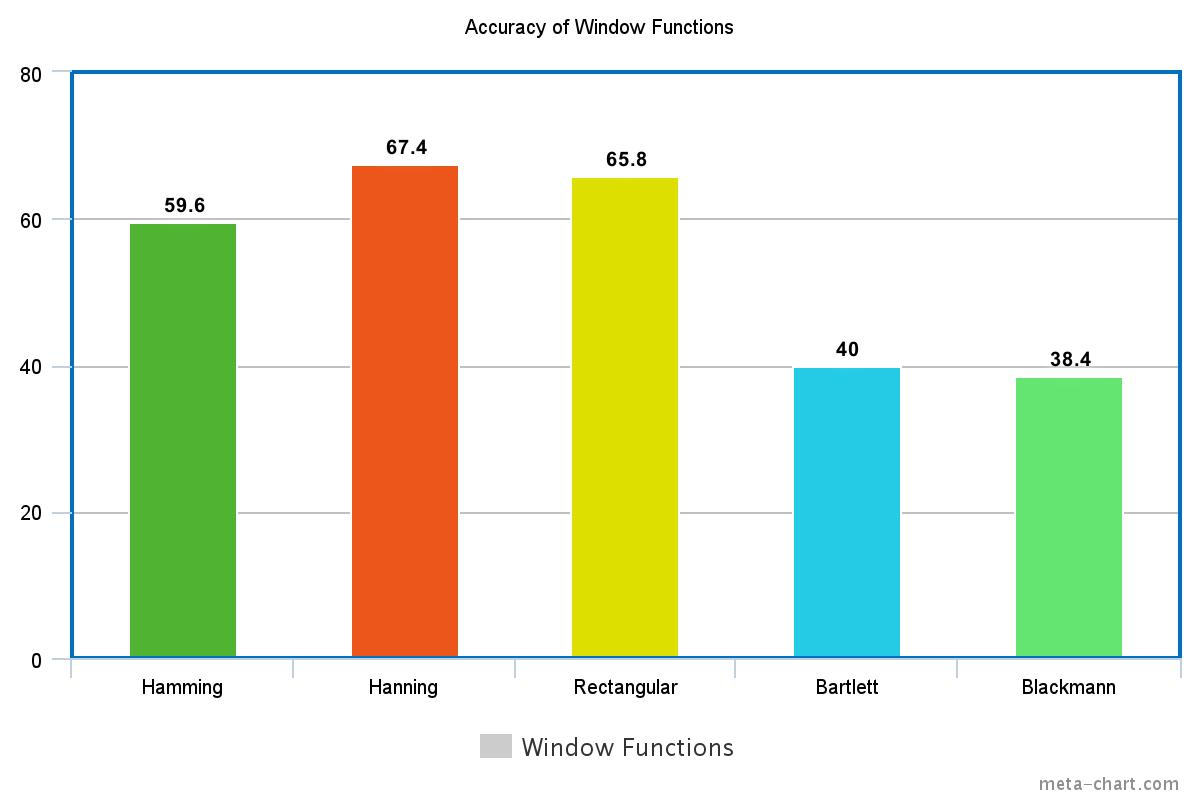
\includegraphics[width=130mm]{resources/mehang/6.3/window}
        \caption{Effect of window functions}
\end{figure}

As seen from the figure, Hanning window gave the best performance. 

\subsubsection{Effect of Frame Size}
The Frame-size needs to be small enough to be statistically invariant but big enough to capture sufficient information. Generally, 20-40ms is taken as the frame size. We tested the frame size according to the number of samples per frame: 512, 1024, 1536 and 2048 samples which correspond to roughly 11.5ms, 23ms, 34.5ms and 46 ms for our songs which have a sampling rate of 44.1 KHz.

\begin{figure}[h!]
        \centering
        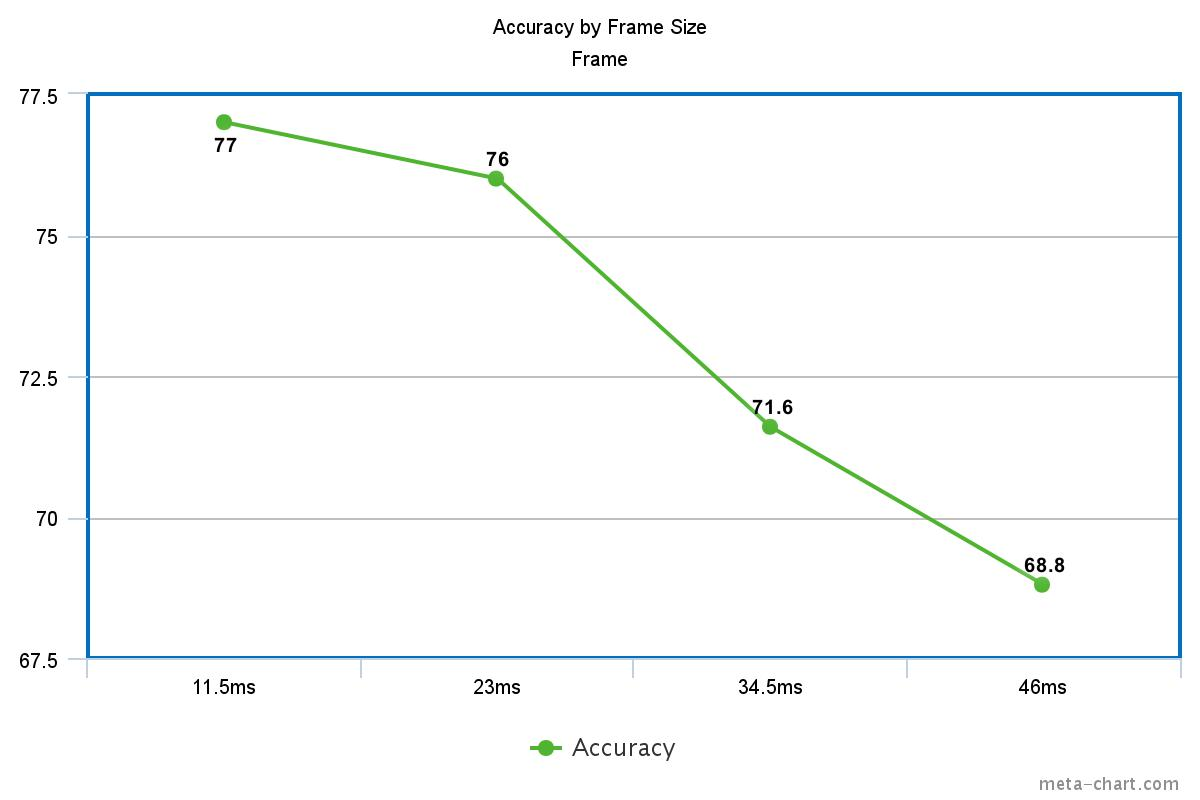
\includegraphics[width=170mm]{resources/mehang/6.3/Frame}
        \caption{Effect of frame size}
\end{figure}

As seen in the figure, frame size of 11.5ms and 23ms performed considerably better than the bigger frame sizes. We chose the 23ms (1024 samples) frame size because the smaller 512 sample frame size would lead to higher number of frames and hence necessitate more computation.

\subsubsection{Effect of Frame Overlap}
We explored four different overlapping schemes: zero per cent, 25 per cent, 50 per cent and 75 per cent overlap.\\
\\
In each of the cases, we received almost the same accuracy (75.4 per cent on No-overlap, 75.8 per cent on Quarter overlap, 76 per cent on half-overlap, and 75.2 per cent on three-quarters overlap). And so, as it seemed to indicate that the overlapping didn’t have any bearing on our results, we chose the less computationally intensive option of using no overlap at all. 

\subsubsection{Effect of Pre-Emphasis}
Pre-emphasis decreased the accuracy from 75.4 per cent to 62.6 per cent.

\newpage
\subsection{Analysis of Features}
\subsubsection{Genre Based Classification}
\begin{table}[h!]
        \caption{Genre classification using ANN}
        \begin{center}
                \begin{tabular}{|l|l|l|l|l|l|l|}
                        \hline Feature & Classical & Hiphop & Jazz & Pop & Rock & Overall\\
                        \hline Spectral Centroid & 47.54 & 11.92 & 11.61 & 51.25 & 18.89 & 28.40\\ 
                        \hline MFCC & 92.45 & 83.42 & 91.57 & 82.98 & 74.44 & 84.20 \\
                        \hline Zero Crossing & 63.29 & 48.31 & 39.83 & 52.65 & 52.00 & 51.20\\
                        \hline Pitch & 37.83 & 15.00 & 34.80 & 61.73 & 1.67 & 28.00\\
                        \hline Compactness & 81.53 & 81.75 & 57.67 & 28.39 & 45.55 & 58.60\\
                        \hline Timbre&
                        6.25
                        &
                        20.00
                        &
                        30.00
                        &
                        20.00
                        &
                        28.46
                        &
                        20.60
                        \\
                        \hline RMS&

                        85.52
                        &
                        34.99
                        &
                        19.85
                        &
                        47.89
                        &
                        70.46
                        &
                        51.20
                        \\

                        \hline Spectral Flux&

                        87.94
                        &
                        26.71
                        &
                        19.77
                        &
                        43.63
                        &
                        57.45
                        &
                        46.40
                        \\

                        \hline Spectral Roll off point&

                        84.10
                        &
                        54.11
                        &
                        22.14
                        &
                        43.74
                        &
                        13.18
                        &
                        41.60
                        \\

                        \hline Spectral Variability&

                        83.10
                        &
                        32.98
                        &
                        25.98
                        &
                        51.24
                        &
                        71.76
                        &
                        52.40
                        \\\hline

                \end{tabular}
        \end{center}
\end{table}

 \begin{table}[h!]
        \caption{Genre classification using SVM}
        \begin{center}
                \begin{tabular}{|l|l|l|l|l|l|l|}
                        \hline

                      Feature 
                      &
                        Classical
                        &
                        Hiphop
                        &
                        Jazz
                        &
                        Pop
                        &
                        Rock
                        &
                        Overall
                        \\\hline
                        Spectral Centroid
                        &
                        58.95
                        &
                        1.11
                        &
                        69.09
                        &
                        7.50
                        &
                        0.00
                        &
                        26.40
\\
\hline
MFCC
&
91.79
&
85.25
&
87.98
&
85.62
&
77.61
&
85.80
\\
\hline

Zero Crossing
&
63.20
&
48.86
&
41.47
&
58.51
&
44.31
&
50.00
\\
\hline

Pitch
&
59.95
&
38.37
&
36.04
&
35.77
&
13.64
&
36.20
\\
\hline

Compactness
&
67.18
&
66.13
&
42.30
&
47.93
&
53.60
&
55.60
\\
\hline

Timbre
&
1.67
&
37.83
&
34.80
&
61.73
&
15.00
&
28.00
\\
\hline

RMS
&
20.00
&
40.00
&
30.00
&
20.00
&
0.00
&
21.60
\\\hline

Spectral Flux
&
59.17
&
10
&
20.91
&
33.06
&
0.00
&
27.20
\\\hline

Spectral Roll off point
&
34.34
&
52.60
&
29.07
&
14.29
&
0.00
&
24.40
\\\hline

Spectral Variability
&
28.46
&
20.00
&
30.00
&
20.00
&
6.25
&
20.60
\\\hline
                 \end{tabular}
        \end{center}
\end{table}

\newpage
\subsubsection{Mood Based Classification}

\begin{table}[h!]
        \caption{Mood classification(Arousal) using ANN}
        \begin{center}
                \begin{tabular}{|l|l|l|l|l|l|l|}
                        \hline
                        Feature
                        &
                        Low Arousal
                        &
                        High Arousal
                        &
                        Overall
                        \\\hline

                        Spectral Centroid
                        &
                        70.07
                        &
                        26.20
                        &
                        50.34
                        \\\hline
                        MFCC
                        &
                        69.32
                        &
                        75.09
                        &
                        71.38
                        \\\hline

                        Zero Crossing
                        &
                        70.70
                        &
                        64.03
                        &
                        67.24
                        \\\hline

                        Pitch
                        &
                        44.27
                        &
                        64.62
                        &
                        54.83
                        \\\hline

                        Compactness
                        &
                        59.73
                        &
                        51.71
                        &
                        57.24
                \\\hline

                Timbre
                &
                58.96
                &
                61.10
                &
                58.28
                \\\hline
                
                RMS
                &
                70.76
                &
                67.28
                &
                68.97
                \\\hline

                Spectral Flux
                &
                76.58
                &
                58.87
                &
                67.93
                \\\hline

                Spectral Roll off point
                &
                50.79
                &
                47.67
                &
                50.34
                \\\hline

                Spectral Variability
                &
                73.28
                &
                62.51
                &
                67.24
                \\\hline
                 \end{tabular}
        \end{center}
\end{table}
\begin{table}[h!]
        \caption{Mood classification(Arousal) using SVM}
        \begin{center}
                \begin{tabular}{|l|l|l|l|l|l|l|}
                        \hline
                        Feature
                        &
                        Low Arousal
                        &
                        High Arousal
                        &
                        Overall
                        \\\hline

                        Spectral Centroid
                        &
                        50.00
                        &
                        50.00
                        &
                        44.14
                        \\\hline

                        MFCC
                        &
                        73.22
                        &
                        71.77
                        &
                        72.41
                        \\\hline

                        Zero Crossing
                        &
                        74.00
                        &
                        67.07
                        &
                        70.69
                        \\\hline

                        Pitch
                        &
                        59.00
                        &
                        55.01
                        &
                        56.55
                        \\\hline

                        Compactness
                        &
                        47.22
                        &
                        78.45
                        &
                        62.76
                        \\\hline

                        Timbre
                        &
                        62.58
                        &
                        53.87
                        &
                        56.55
                        \\\hline

                        RMS
                        &
                        50.00
                        &
                        50.00
                        &
                        42.76
                        \\\hline

                        Spectral Flux
                        &
                        40.00
                        &
                        60.00
                        &
                        45.86
                        \\\hline

                        Spectral Roll off point
                        &
                        70.00
                        &
                        30.00
                        &
                        41.38
                        \\\hline

                        Spectral Variability
                        &
                        50.00
                        &
                        50.00
                        &
                        40.00
                        \\\hline

                 \end{tabular}
        \end{center}
\end{table}

\vspace{30mm}
\begin{table}[h!]
        \caption{Mood classification(Valence) using ANN}
        \begin{center}
                \begin{tabular}{|l|l|l|l|l|l|l|}
                        \hline
                        
                        Feature
                        &
                        Low Valence
                        &
                        High Valence
                        &
                        Overall\\\hline

                        Spectral Centroid
                        &
                        37.69
                        &
                        60.63
                        &
                        51.38
                        \\\hline

                        MFCC
                        &
                        60.04
                        &
                        65.45
                        &
                        63.79
                        \\\hline

                        Zero Crossing
                        &
                        62.74
                        &
                        57.80
                        &
                        59.66
                        \\\hline

                        Pitch
                        &
                        66.29
                        &
                        35.46
                        &
                        50.69
                        \\\hline

                        Compactness
                        & 
                        50.67
                        &
                        58.79
                        &
                        52.76
                        \\\hline

                        Timbre
                        &
                        61.75
                        &
                        57.69
                        &
                        56.90
                        \\\hline

                        RMS
                        &
                        63.85
                        &
                        44.87
                        &
                        53.79
\\\hline

                        Spectral Flux
                        &
                        70.19
                        &
                        47.50
                        &
                        59.31
                        \\\hline

                        Spectral Roll off point
                        &
                        57.56
                        &
                        44.94
                        &
                        48.28
                        \\\hline

                        Spectral Variability
                        &
                        63.99
                        &
                        45.13
                        &
                        51.03
                        \\\hline


                 \end{tabular}
        \end{center}
\end{table}
\begin{table}[h!]
        \caption{Mood classification(Valence) using SVM}
        \begin{center}
                \begin{tabular}{|l|l|l|l|l|l|l|}
                        \hline

                        Feature
                        &
                        Low Valence
                        &
                        High Valence
                        &
                        Overall
                        \\\hline

                        Spectral Centroid
                        &
                        40.00
                        &
                        60.00
                        &
                        44.83
                        \\\hline

                        MFCC
                        &
                        45.37
                        &
                        72.06
                        &
                        58.62
                        \\\hline

                        Zero Crossing
                        &
                        70.34
                        &
                        52.46
                        &
                        60.34
                        \\\hline

                        Pitch
                        &
                        53.56
                        &
                        52.53
                        &
                        49.66
                        \\\hline

                        Compactness
                        &
                        57.25
                        &
                        62.40
                        &
                        58.97
                        \\\hline

                        Timbre
                        &
                        60.50
                        &
                        61.19
                        &
                        60.34
                        \\\hline

                        RMS
                        &
                        50.00
                        &
                        50.00
                        &
                        44.83
                        \\\hline

                        Spectral Flux
                        &
                        60.00
                        &
                        40.00
                        &
                        40.34
                        \\\hline

                        Spectral Roll off point
                        &
                        60.00
                        &
                        40.00
                        &
                        41.72
                        \\\hline

                        Spectral Variability
                        &
                        50.00
                        &
                        50.00
                        &
                        41.83
                        \\\hline

                 \end{tabular}
        \end{center}
\end{table}

\newpage
\newpage
\newpage
\subsubsection{Effect of Number of MFCCs on Result}
\begin{figure}[h!]
        \centering
        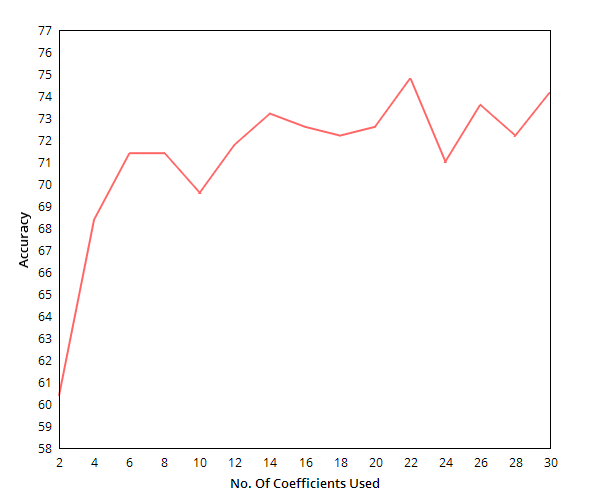
\includegraphics[width=170mm]{resources/mehang/6.4/MFCC_Num}
        \caption{Effect of number of MFCCs on result}
\end{figure}
The results indicate that once we use more than 10 MFCC Coefficients, the accuracy plateaus and doesn’t increase at all. So, using around 15 coefficients is found to be good enough for the problem domain.  

\newpage
\subsection{Analysis of Classifiers}
\subsubsection{SVM}
\paragraph{Selection of Kernels.}
\begin{figure}[h!]
        \centering
        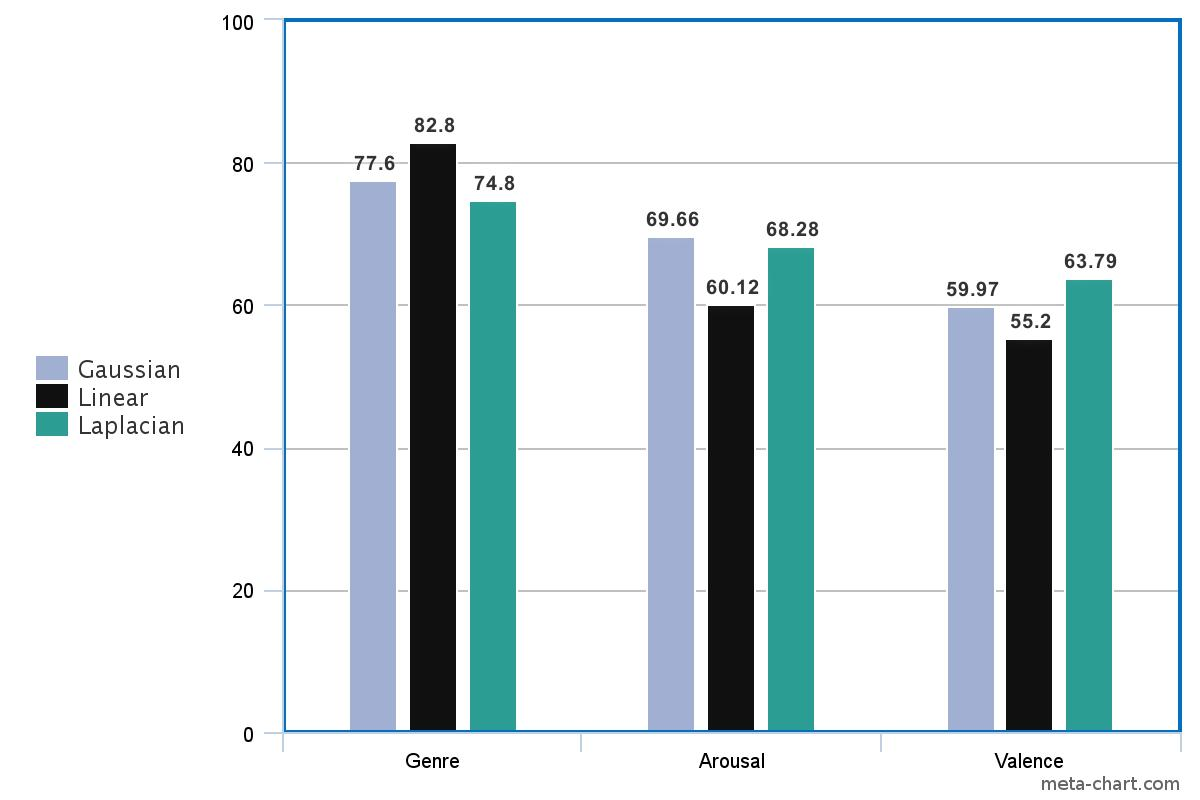
\includegraphics[width=170mm]{resources/mehang/6.5/SVM_Kernel}
        \caption{SVM Kernel}
\end{figure}

Linear Kernel performed best for the Genre Classification Problem and so we selected it for Genre Classification.\\
\\
As for the Mood Classification problem, both Gaussian and Laplacian out-performed the Linear Kernel in both arousal and valence classification. So, we selected Laplacian Kernel (based on its slightly superior performance) as our Kernel for Mood Classification.

\paragraph{Effect of Learning Iterations.}
We tested three iteration values to train SVM: one, 10 and 100.\\ 
\\
For Genre Classification, all three of them resulted in a similar performance of around 77 per cent accuracy.\\ 
\\
For Arousal, the performance increased when going from one (61 per cent) to 10 (69 per cent) iterations but increasing it further to 100 iterations didn’t increase the performance. We still received an accuracy of around 69 per cent.

\subsubsection{ANN}
\paragraph{Activation and Error Functions.}
We tried out two sets of Activation and Error Functions for the Neural Network with a 1000 iteration training.\\
\\
The results are given below:\\

\begin{table}[h!]
        \caption{Genre}
        \begin{center}
            \begin{tabular}{|p{8cm}|l|l|l|}
                        \hline

                        \textbf{Functions}
                        &
                        \textbf{Accuracy(percent)}
                        &
                        \textbf{Precision}
                        &
                        \textbf{Recall}
                        \\\hline

Cross Entropy Error with Softmax Activation
&
85.80
&
0.92
&
0.92
\\\hline

Least Mean Squares Error with Logistic Sigmoid Activation 
&
83.60
&
0.87
&
0.89
\\\hline
                 \end{tabular}
        \end{center}
\end{table}
So, the first combination slightly outperforms the second in all three metrics. 
\begin{table}[h!]
        \caption{Arousal}
        \begin{center}
            \begin{tabular}{|p{8cm}|l|l|l|}
                        \hline

                        \textbf{Functions}
                        &
                        \textbf{Accuracy(per cent)}
                        &
                        \textbf{Precision}
                        &
                        \textbf{Recall}
                        \\\hline

                        Cross Entropy Error with Softmax Activation
                        &
                        69.31
                        &
                        0.72
                        &
                        0.64
                        \\\hline
                        
                        Least Mean Squares Error with Logistic Sigmoid Activation 
                        &
                        70.34
                        &
                        0.72
                        &
                        0.65
                        \\\hline

                 \end{tabular}
        \end{center}
\end{table}
\begin{table}[h!]
        \caption{Valence}
        \begin{center}
            \begin{tabular}{|p{8cm}|l|l|l|}
                        \hline

                        \textbf{Functions}
                        &
                        \textbf{Accuracy(per cent)}
                        &
                        \textbf{Precision}
                        &
                        \textbf{Recall}
                        \\\hline

                        Cross Entropy Error with Softmax Activation
                        &
                        63.27
                        &
                        0.67
                        &
                        0.60
                        \\\hline
                        
                        Least Mean Squares Error with Logistic Sigmoid Activation 
                        &
                        64.31
                        &
                        0.68
                        &
                        0.60
                        \\\hline

                 \end{tabular}
        \end{center}
\end{table}

Here, the two combinations are almost inseparable in terms of performance. 

\paragraph{Number of Nodes in Hidden Layer:}

We used only one hidden layer as it should be enough for our problem domain. 
As seen in the figure, for any number of hidden numbers after six or so, we get almost the same accuracy. As a rule of thumb, it is usually recommended that the number of nodes be around the mean of the number of inputs and outputs, so we chose 30 as our final number of hidden nodes.\\

\begin{figure}[h!]
        \centering
        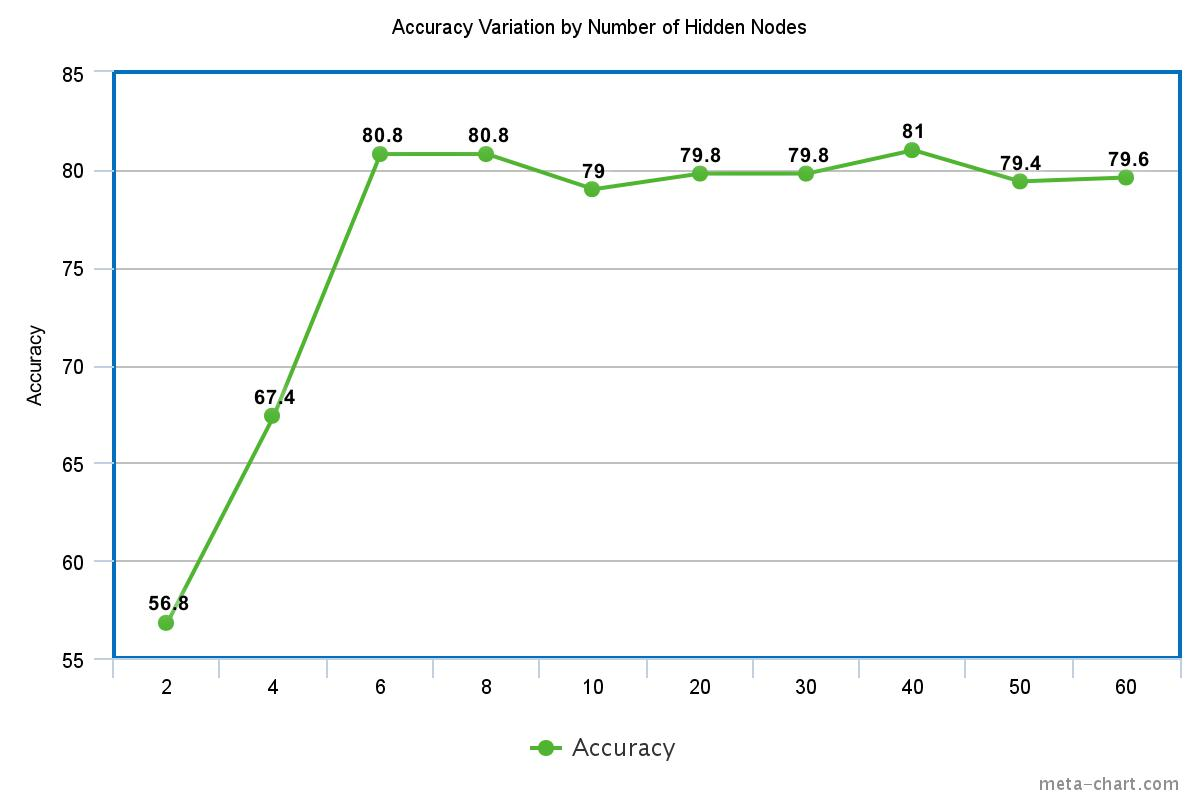
\includegraphics[width=170mm]{resources/mehang/6.5/ANN_HiddenNodes}
        \caption{Effect of number of hidden nodes}
\end{figure}

The number of nodes had minimal effect in regard to mood classification. 

\paragraph{Number of Iterations:}
As seen in the figure, for genre classification, the number of iterations has an effect on the accuracy up to a certain point (around 20 iterations).\\

\begin{figure}[h!]
        \centering
        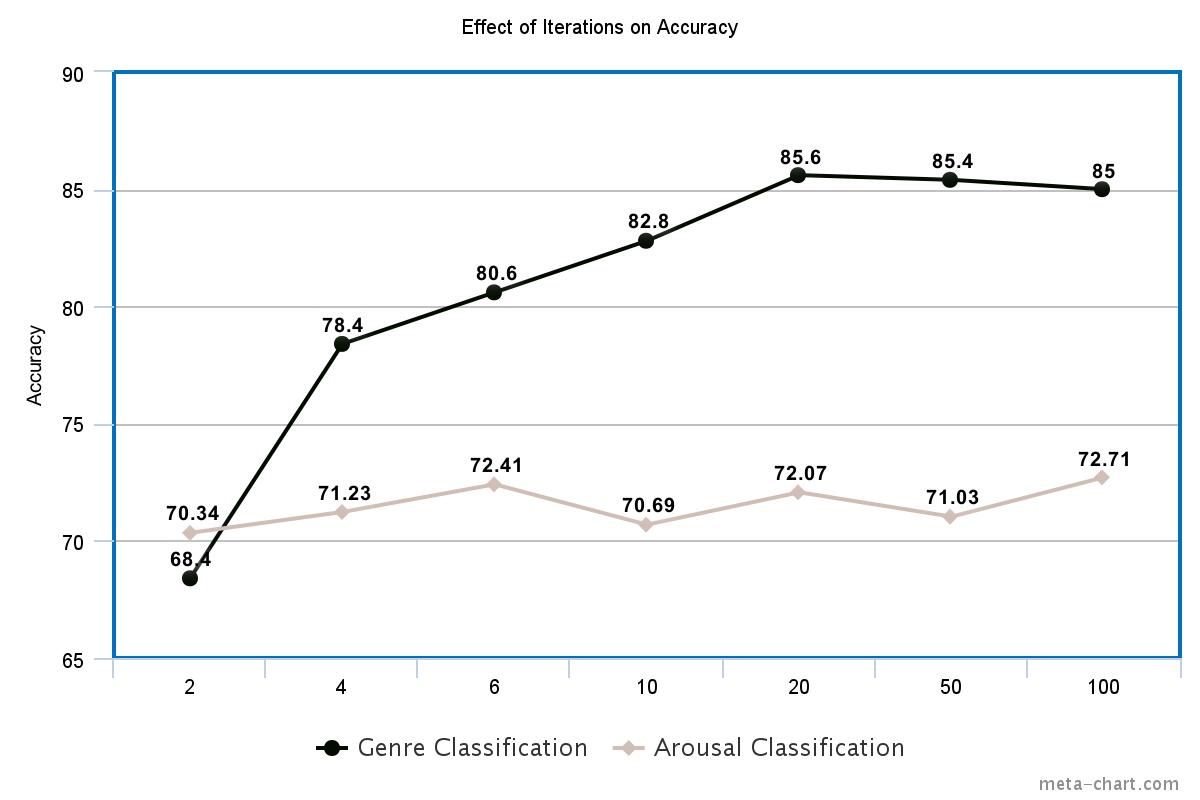
\includegraphics[width=130mm]{resources/mehang/6.5/ANN_Iterations}
        \caption{Effect of number of iterations}
\end{figure}

As for Arousal, the increase in iterations had no effect on the accuracy. 

\newpage
\paragraph{Learning Rate:}

A learning rate of 0.1 was enough to get a decent amount of accuracy. A lower rate than that affected the accuracy while a higher rate didn’t have any influence at all.
\begin{figure}[h!]
        \centering
        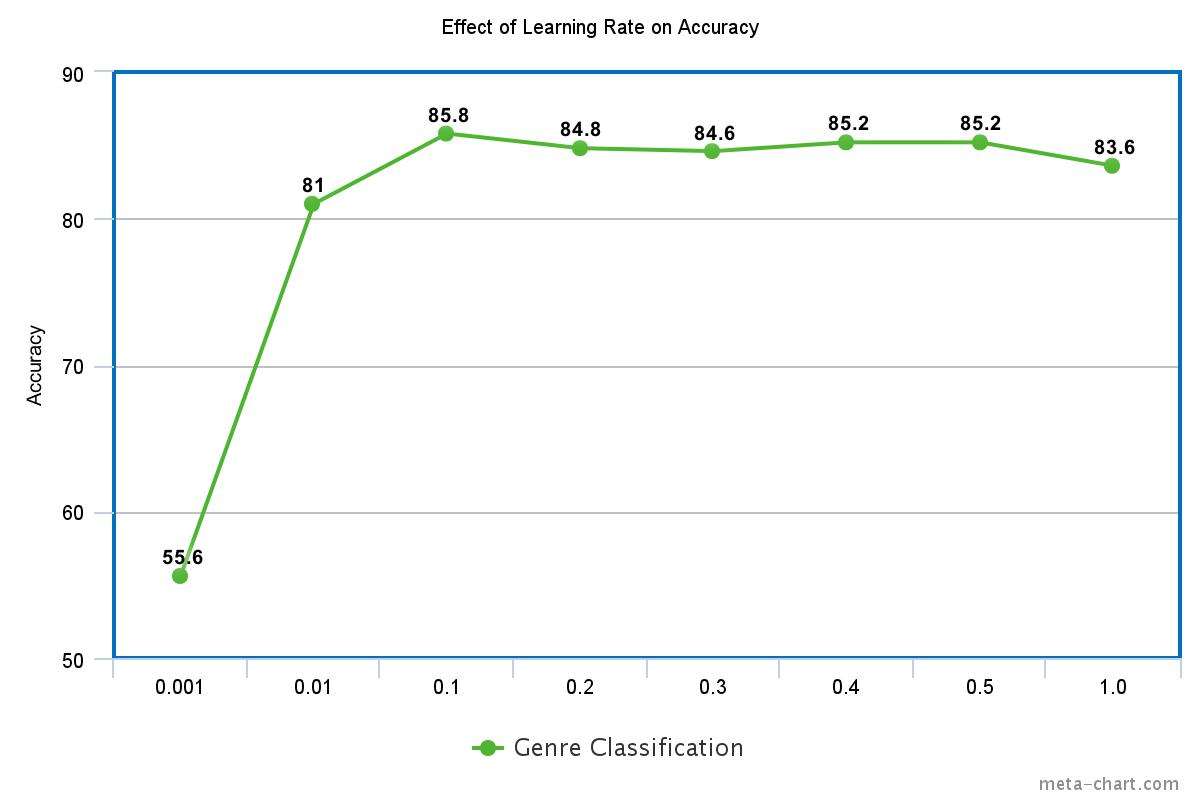
\includegraphics[width=130mm]{resources/mehang/6.5/ANN_Learning}
        \caption{Effect of learning rate}
\end{figure}
\newpage
\subsection{Final Results}
\subsubsection{Genre Classification}
\begin{figure}[h!]
        \centering
        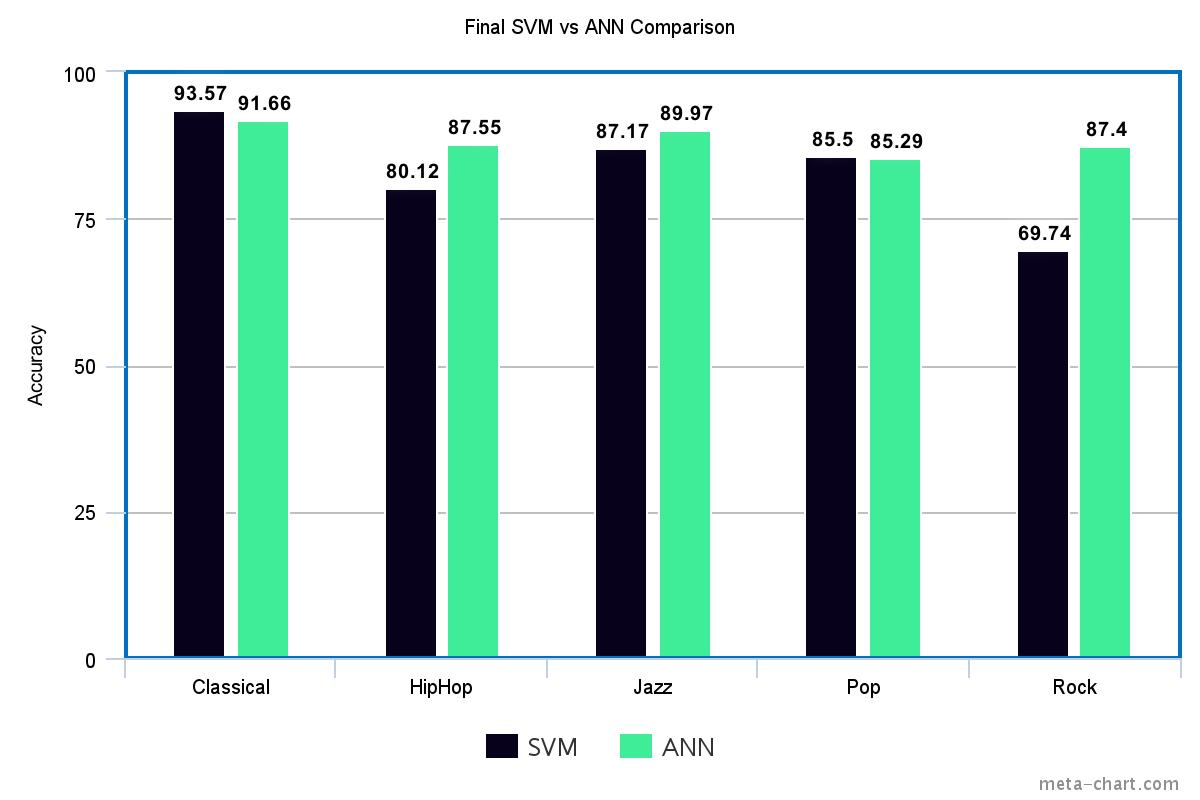
\includegraphics[width=130mm]{resources/mehang/6.6/FinalSVMANNGenre}
        \caption{Final SVM and ANN comparision based on genre}
\end{figure}

\begin{table}[h!]
        \caption{Genre classification performance measure}
        \begin{center}
                \begin{tabular}{|l|l|l|l|l|}
                        \hline

                        Classifier
                        &
                        Precision 
                        &
                        Recall 
                        &
                        F-Measure
                        &
                        Accuracy
                        \\\hline

                        SVM
                        &
                        0.87
                        &
                        0.94
                        &
                        0.89
                        &
                        83.00
                        \\\hline


                        ANN
                        &
                        0.94
                        &
                        0.92
                        &
                        0.92
                        &
                        88.80
                        \\\hline
                \end{tabular}
        \end{center}
\end{table}

For our final model we used ANN with these feature: MFCC, Spectral Centroid, Zero Crossing, Compactness and RMS.

\begin{table}[h!]
        \caption{Genre classification confusion matrix}
        \begin{center}
                \begin{tabular}{|l|l|l|l|l|l|}
                        \hline
                        &
                        Classical
                        &
                        Hiphop
                        &
                        Jazz
                        &
                        Pop
                        &
                        Rock
                        \\\hline

                        Classical
                        &
                        93
                        &
                        1
                        &
                        4
                        &
                        0
                        &
                        2
                        \\\hline

                        Hiphop
                        &
                        0
                        &
                        88
                        &
                        0
                        &
                        3
                        &
                        9
                        \\\hline


                        Jazz
                        &
                        5
                        &
                        0
                        &
                        90
                        &
                        1
                        &
                        4
                        \\\hline


                        Pop
                        &
                        2
                        &
                        7
                        &
                        0
                        &
                        86
                        &
                        5
                        \\\hline

                        Rock
                        &
                        0
                        &
                        4
                        &
                        4
                        &
                        5
                        &
                        87
                        \\\hline
                \end{tabular}
        \end{center}
\end{table}

\subsubsection{Mood Classification}
\begin{figure}[h!]
        \centering
        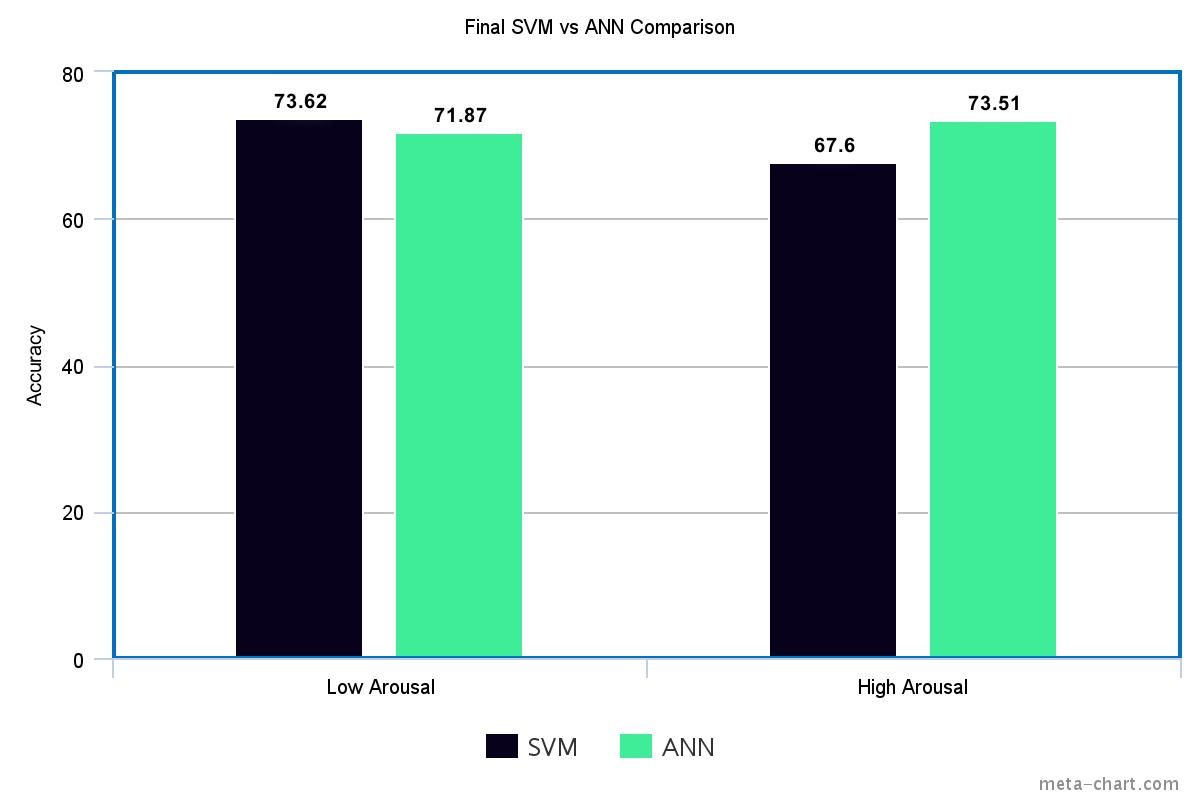
\includegraphics[width=130mm]{resources/mehang/6.6/FinalSVMANNArousal}
        \caption{Final SVM and ANN comparision based on arousal}
\end{figure}

\begin{table}[h!]
        \caption{Arousal classification performance measure}
        \begin{center}
                \begin{tabular}{|l|l|l|l|l|}
                        \hline

                        Classifier
                        &
                        Precision 
                        &
                        Recall 
                        &
                        F-Measure
                        &
                        Accuracy
                        \\\hline

                        SVM
                        &
                        0.70
                        &
                        0.74
                        &
                        0.72
                        &
                        70.69
                        \\\hline

                        ANN
                        &
                        0.75
                        &
                        0.72
                        &
                        0.72
                        &
                        73.10
                        \\\hline

                \end{tabular}
        \end{center}
\end{table}

For our final model we used ANN with these feature: Spectral centroid, MFCC, Zero Crossing, Compactness, Rhythm, Spectral Flux, RMS and Spectral Variability.

\begin{table}[h!]
        \caption{Arousal classification confusion matrix}
        \begin{center}
                \begin{tabular}{|l|l|l|}
                        \hline
                        &
                        Low Arousal
                        &
                        High Arousal
                        \\\hline

                        Low Arousal
                        &
                        105
                        &
                        40
                        \\\hline

                        High Arousal
                        &
                        38
                        &
                        107
                        \\\hline
                \end{tabular}
        \end{center}
\end{table}

\begin{figure}[h!]
        \centering
        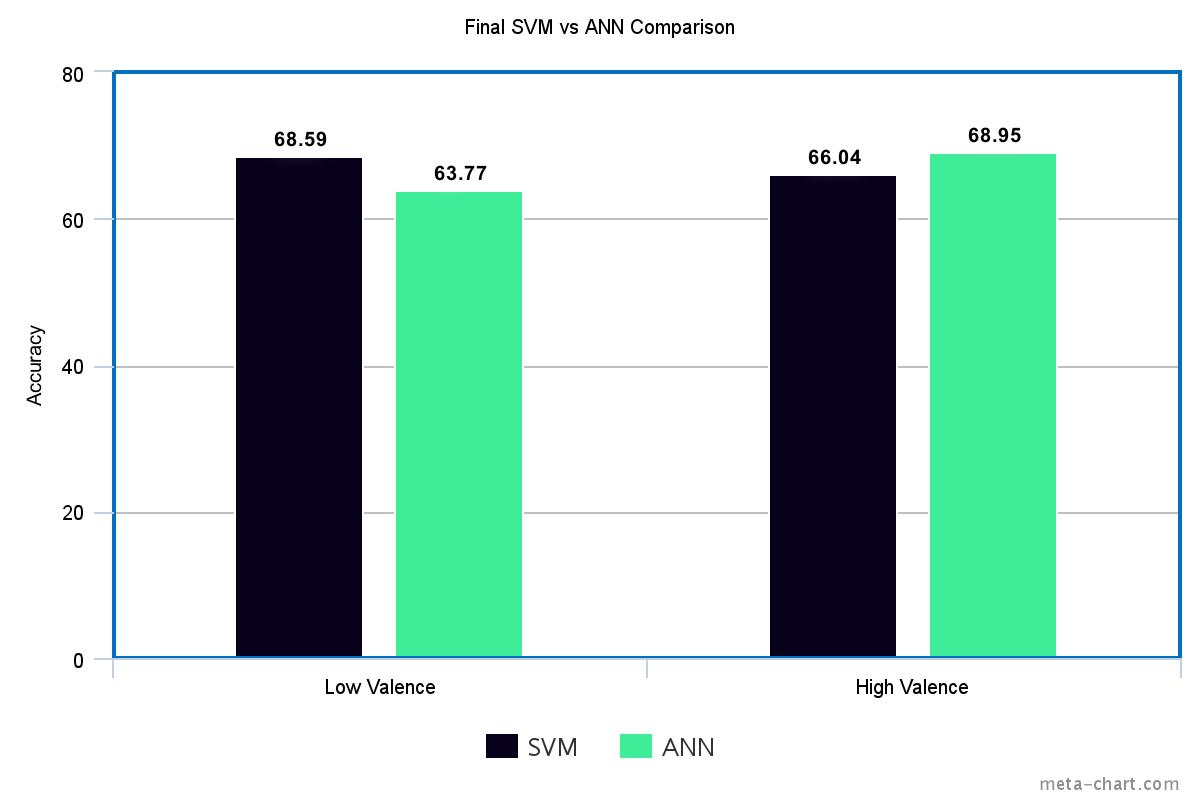
\includegraphics[width=130mm]{resources/mehang/6.6/FinalSVMANNValence}
        \caption{Final SVM and ANN comparision based on valence}

\end{figure}

\begin{table}[h!]
        \caption{Valence performance measure}
        \begin{center}
                \begin{tabular}{|l|l|l|l|l|}
                        \hline

                        Classifier
                        &
                        Precision 
                        &
                        Recall 
                        &
                        F-Measure
                        &
                        Accuracy
                        \\\hline

                        SVM
                        &
                        0.68
                        &
                        0.69
                        &
                        0.68
                        &
                        67.59
                        \\\hline

                        ANN
                        &
                        0.68
                        &
                        0.64
                        &
                        0.65
                        &
                        67.24
                        \\\hline

                \end{tabular}
        \end{center}
\end{table}

For our final model we used ANN with these feature: Spectral centroid, MFCC, Zero Crossing, Compactness, Rhythm, Spectral Flux, RMS and Spectral Variability.

\begin{table}[h!]
        \caption{Valence confusion matrix}
        \begin{center}
                \begin{tabular}{|l|l|l|}
                        \hline

                        &
                        Low Valence
                        &
                        High Valence
                        \\\hline

                        Low Valence
                        &
                        95
                        &
                        52
                        \\\hline

                        High Valence
                        &
                        43
                        &
                        100
                        \\\hline

                \end{tabular}
        \end{center}
\end{table}

\subsection{Problems and Solutions}
\subsubsection{Solved Problems}
\begin{enumerate}[(i)]
        \item \textbf{Mp3 Decoding:}The Mp3 file format uses various lossy compression techniques that allows it to store audio data in a compact and efficient manner. That however means that its headers and file formats are pretty complicated and decoding them would require a substantial amount of work. So, we had problems reading and decoding the Mp3 file format.\\ 
                \\
                We solved it by using the Mp3SPI library which read and gave us the samples of the mp3 files.
        \item \textbf{Feature Integration:}We had trouble deciding ways in which we could integrate the different song features into a single feature-set that could represent the song. This was complicated by the fact that the features all varied in length, range as well as magnitudes. 
                In the end, we concatenated the features into a single feature vector. However, by storing their means and standard deviation and normalizing them before usage, we minimized the effects of one feature over the others. 
        \item \textbf{Feature and Model Persistence:}We needed a way to store the extracted features and also the trained models. Doing so in a simple file or creating our own writer/parser for various appropriate formats would be error-prone and take up a lot of our time. 
                So, we used GSON and XStream to store and also read them as JSON and XML files respectively. 
        \item \textbf{Pitch Extraction:}Pitch is the perceived fundamental frequency and hence it is subjective. So, there is no definite mathematical formulae or methods to represent or calculate it. 
                So, we used the TarsosDSP library to extract pitch. 
\end{enumerate}

\subsubsection{Unsolved Problems}
\begin{enumerate}[(i)]
        \item \textbf{Distance Measure for Songs:} One way to achieve song clustering or even classification is to develop distance measures to figure out the ''distance'' or difference between any two given songs. So, we tried to do the same. However, our initial attempts at using a simple Euclidean Distance measure didn’t prove successful and later attempts using Gaussian Mixture Models proved to be too computationally intensive to be useful. 
        \item \textbf{Heap Error on Long Songs:}Due to lack of memory optimization we run into a Heap error when processing songs longer than about six minutes. This might be solved by better profiling of the memory used or by using shorter sections of songs for classification.
\end{enumerate}


